\section{Experimental Setup}
The setup as drawn in the instructions is shown in \cref{fig:setup1}. In addition to this our experimental setup with the apparature is shown in \cref{fig:setup}. 
The light source For the beamsize we used a collimating slit of five variable widths.

\begin{figure}[h]
    \centering
    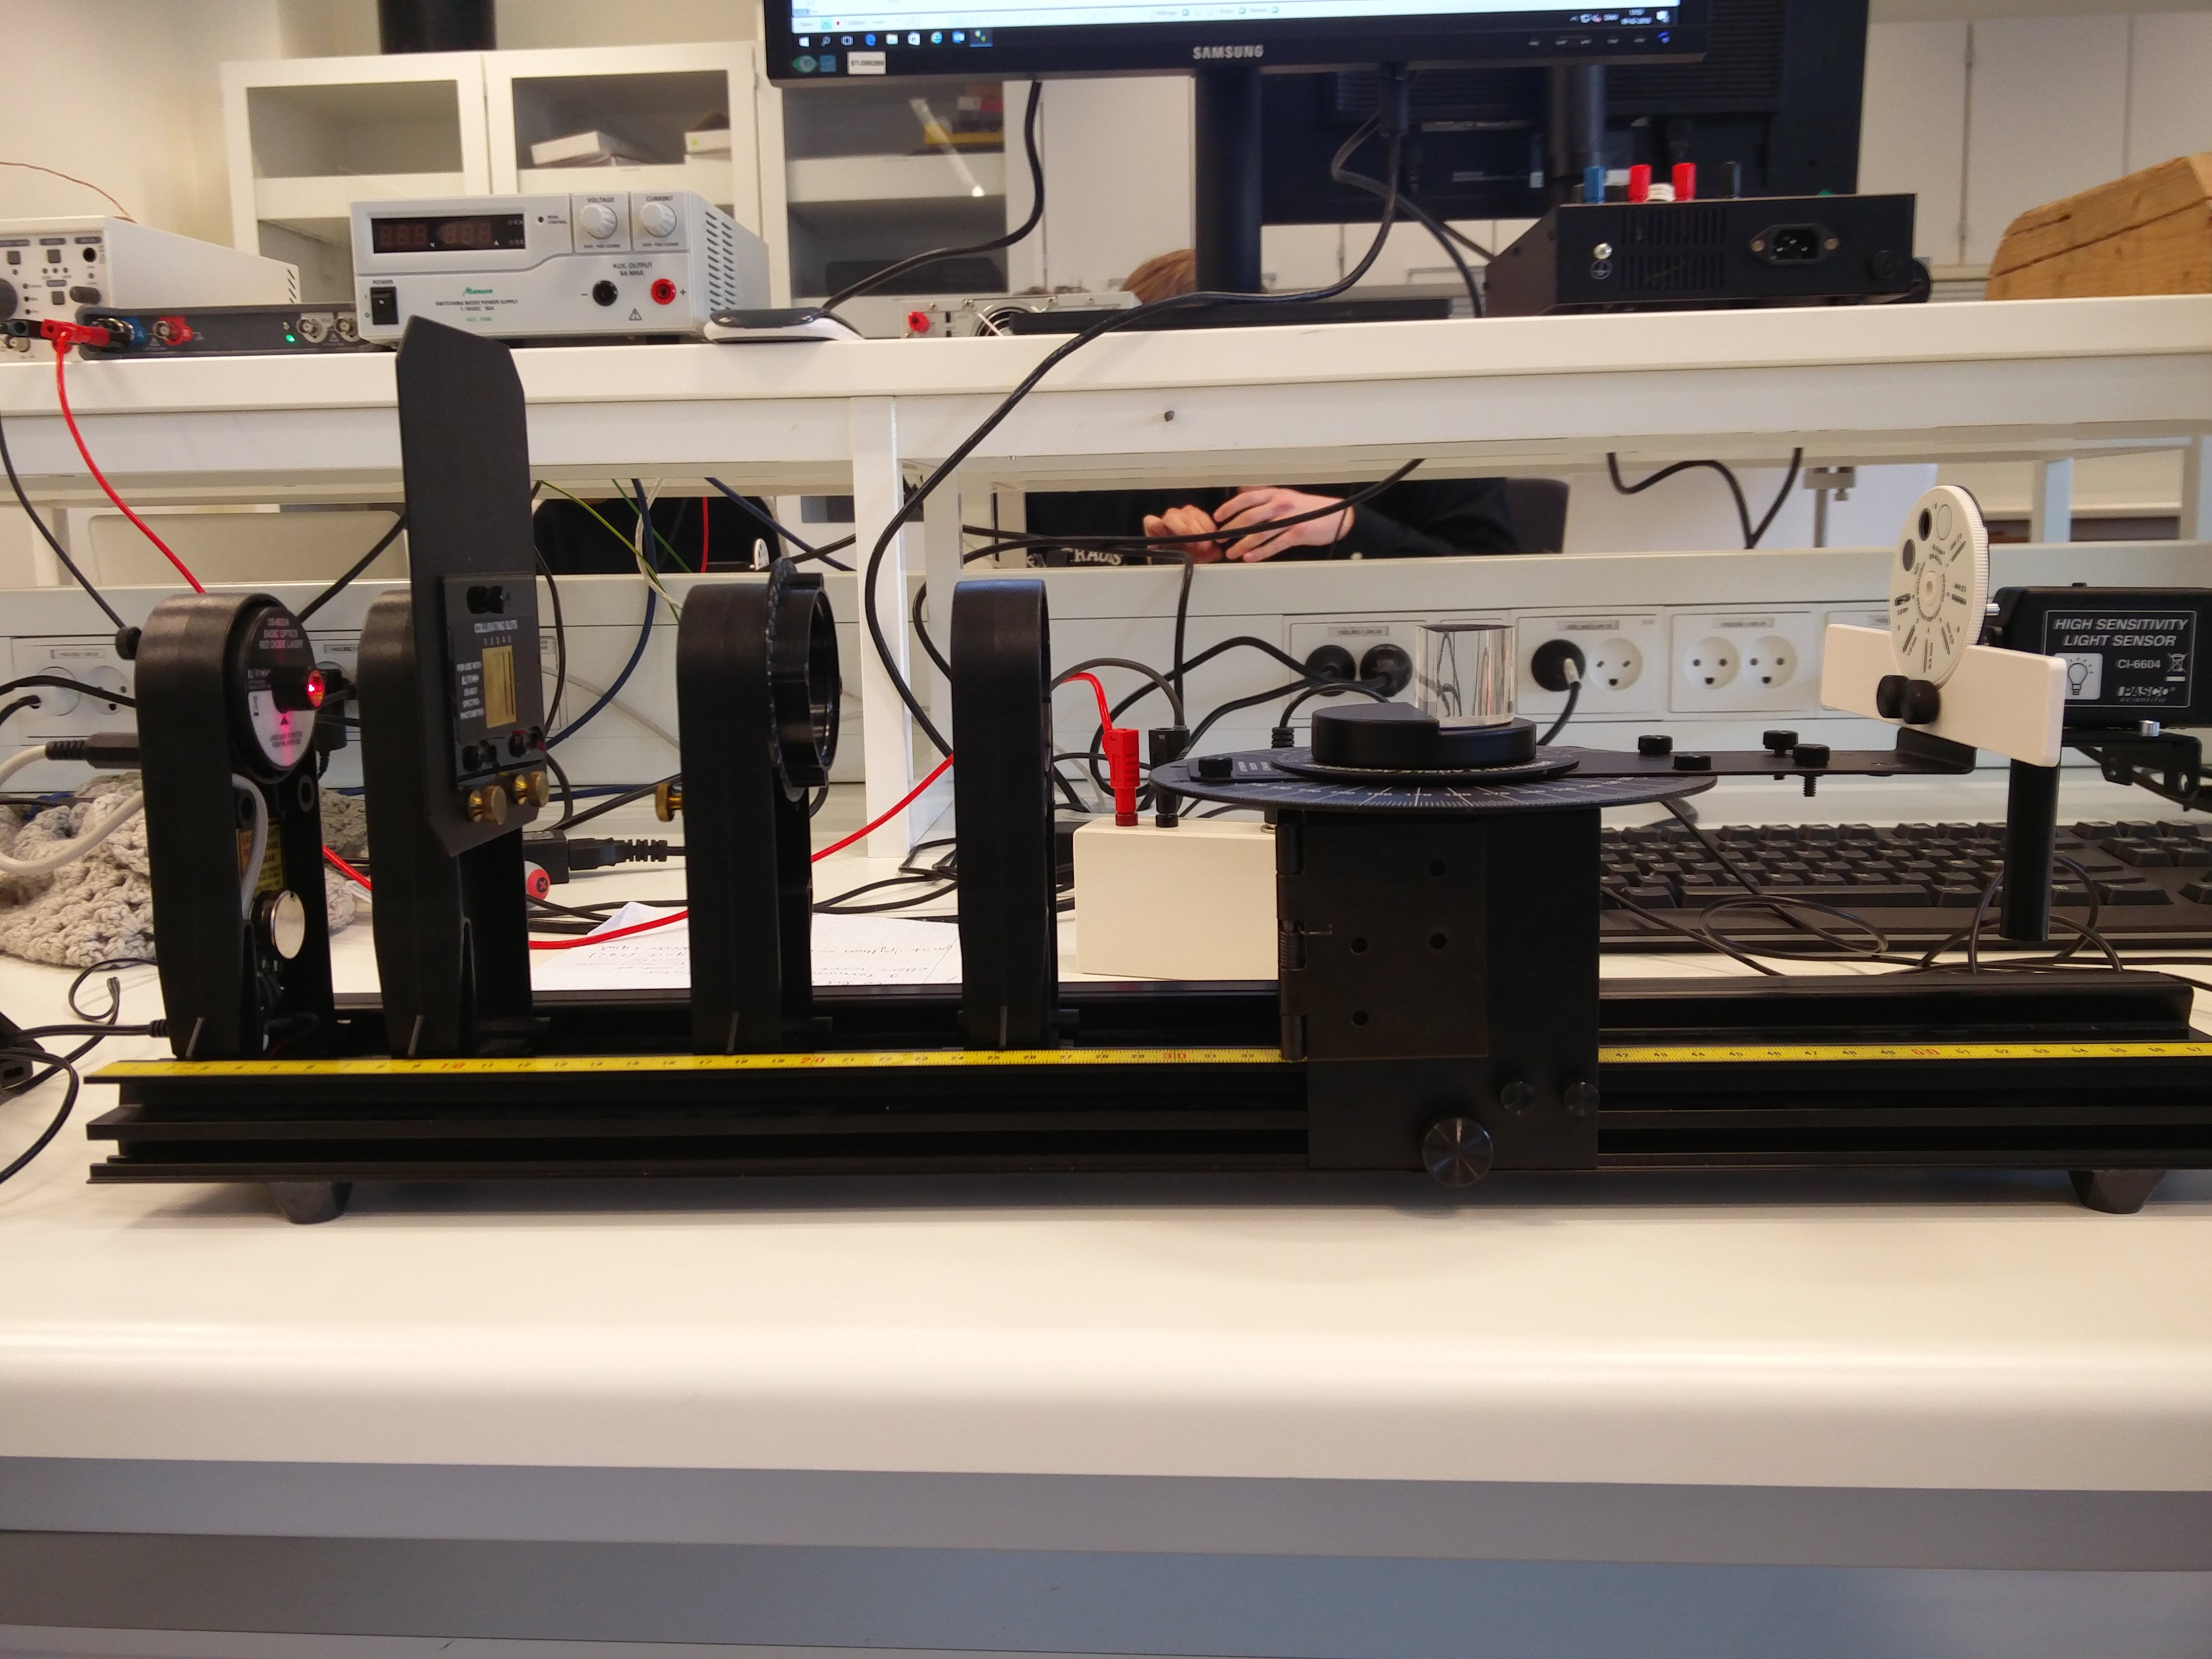
\includegraphics[trim={0 25cm 0 20cm}, clip, width=\columnwidth]{setup}
\caption{Experimental setup. From left to right: Red diode laser, collimating slit with customizable slitwidth, polarizer with rotational mount, collimating lense, glass, polarizer, High sensitivity light sensor (connected to PicoScope)}
    \label{fig:setup}
\end{figure}

\begin{figure}[h]
    \centering
    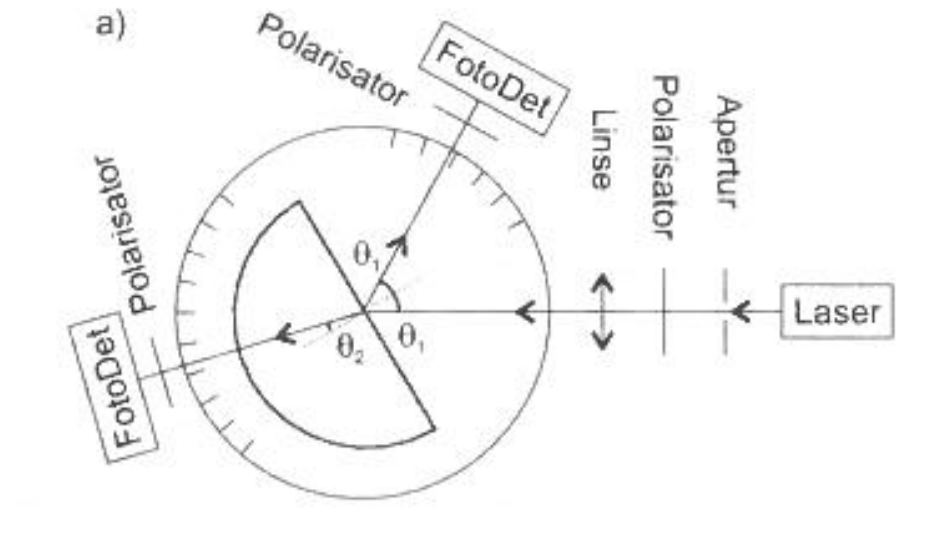
\includegraphics[width = \columnwidth]{setup1}
    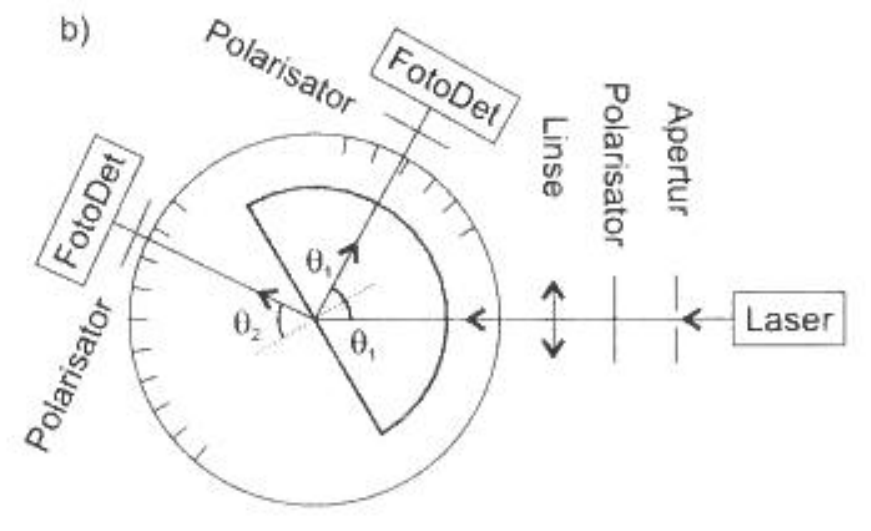
\includegraphics[width = \columnwidth]{setup2}
    \caption{a) and b) for beam from air toward glass and glass toward air respectively}
    \label{fig:setup1}
\end{figure}

\subsection{Procedure}
Firstly the setup must be carefully aligned in order to maximize the amount of laser light hitting the detector.  We assured that the laser went as directly as possible through one of the first $3$ collimating slits. Afterwards one must assure that the light from the laser is equally polarized. This is done by leaving the square polarization filter in front of the detector while tuning the polarizer at different angles while observing the intensity of the beam at PicoScope. One observes that dependent on the choice of $s$- or $p$-polarization there is a minima/maxima of the intensity at $0$ and $90$ degrees respectively. The polarizer is then set to $45$ degrees in order to get equally polarized light. There is a slight uncertainty in to the exact $50/50$ position of the polarizer as the minima and maxima of the polarized light were quite broad.

We did seperate measurements for transmission and reflection coefficients. To measure the reflection coefficient we measured the beams that were in area between our laser and our dielectric (of course not the incoming laser beam), and for the transmission we did our measurements on the part of the beam that was refracted to the area between the origin position of the detector and the dielectric. The polarization of the light was changed by tilting the square polarization filter by $90$ degrees. The measurement procedure we used were as follows:

Align the outer disk such that the white line on the measurement apparatus is aligned with either $0$ or $180$ degress. Make sure that the dielectric is placed in the center of the inner desk. Place the inner disk such that $0$ degrees aligns with $0$ degrees on the outer disk.

Move the inner disk to the desired angular displacement. Move the detector to capture the transmitted or reflected beam respectively. Make sure that the beam of the given polarization is intense enough by tuning the intensity of the detector. The intensity may not be higher than $\SI{5}{\volt}$ at $90$ degrees for the reflected beam and at $0$ degrees for the transmitted beam, as the detector does not tolerate voltages higher than $\SI{5}{\volt}$. 

The beam can be adjusted up and down on the laser to hit the detector optimally. Note the angle on the outer disk and the intensity of the beam in PicoScope.

Turn off PicoScope and measure the background intensity at the given angle of the detector and note it.

Reset experiement to original outer/inner disk configuration before doing a new measurement.

Make sure to measure the intensity at $90$ degrees for reflection and $0$ degrees for transmission. 
